%░▒█▀▀▀█░▒█▀▀▄░▒█▀▀▀█░▒█▀▀▀░▒█▀▀▄░▒█░░▒█░█▀▀▄░▀▀█▀▀░▀█▀░▒█▀▀▀█░▒█▄░▒█░▒█▀▀▀█
%░▒█░░▒█░▒█▀▀▄░░▀▀▀▄▄░▒█▀▀▀░▒█▄▄▀░░▒█▒█░▒█▄▄█░░▒█░░░▒█░░▒█░░▒█░▒█▒█▒█░░▀▀▀▄▄
%░▒█▄▄▄█░▒█▄▄█░▒█▄▄▄█░▒█▄▄▄░▒█░▒█░░░▀▄▀░▒█░▒█░░▒█░░░▄█▄░▒█▄▄▄█░▒█░░▀█░▒█▄▄▄█
%.:..:..:..:..:..:..:..:..:..:..:..:..:..:..:..:..:..:..:..:.
\section{Observations}
%,;,,;,,;,,;,,;,,;,,;,,;,,;,,;,,;,,;,,;,,;,,;,,;,,;,,;,,;,,;,
\subsection{Outcome reliability and simulated bits}
It was found through innumerable iterations that the resulting bit error performance curves' consistency was commensurate with the number of simulated bits being transmitted through the system. This is due to the following:
\begin{itemize}
	\item Statistically, large populations eliminate the spurious effects of randomness, as highlighted in the challenges section.
		\item Higher bit counts allow for smaller BER values, which in turn facilitate continuous, deeper and more accurate BER performance curves.
\end{itemize}
\begin{figure}[!h]
	\centerline{\resizebox{!}{0.6\textheight}{\includegraphics{Graphics/Conclusion/databits.pdf}}}
	\caption{Effect of databits on BER performance}
	\label{res:fig:bervariation}
\end{figure}

%,;,,;,,;,,;,,;,,;,,;,,;,,;,,;,,;,,;,,;,,;,,;,,;,,;,,;,,;,,;,
\subsection{Effect of \emph{K} on BER curve}
It was observed that as \(K \to \infty\), the BER performance curve for the Rician channel model approximates an AWGN channel while as \(K \to -\infty\), the Rician channel's error performance approximates a Rayleigh channel model.
\begin{figure}[!h]
	\centerline{\resizebox{!}{0.5\textheight}{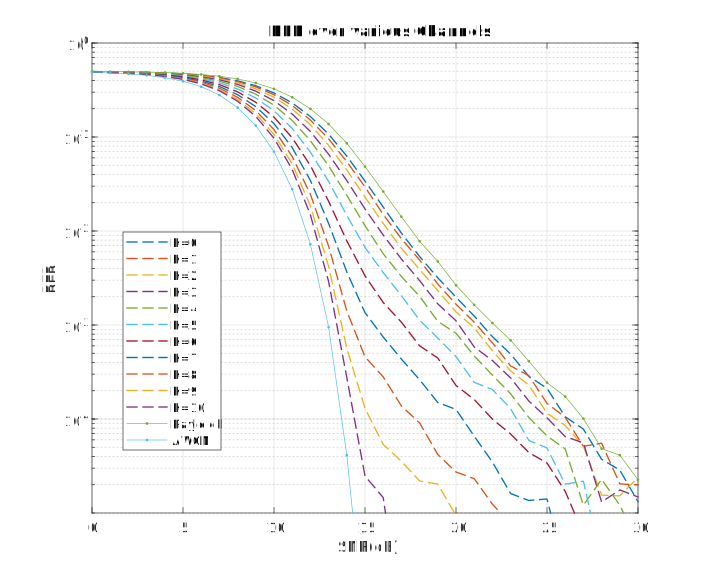
\includegraphics{Graphics/Results/Curves/AllOfThem.pdf}}}
	\caption{Effect of K on BER performance}
	\label{res:fig:Kvariation}
\end{figure}

